\documentclass[a4paper, 11pt, notitlepage, english]{article}

\usepackage{babel, textcomp}
\usepackage[latin1]{inputenc}
\usepackage[T1]{fontenc, url}
\usepackage{amsmath, amssymb}
\usepackage{amsbsy, amsfonts}
\usepackage{graphicx, color, xcolor}
\usepackage{framed, parskip}
\usepackage{flafter, caption, multicol}
\usepackage{verbatim, listings, fancyvrb}
\usepackage{mathrsfs}

\usepackage{geometry}
\geometry{headheight=0.01mm}
\geometry{top=24mm, bottom=29mm, left=39mm, right=39mm}

\renewcommand{\arraystretch}{2}
\setlength{\tabcolsep}{10pt}
\makeatletter
\renewcommand*\env@matrix[1][*\c@MaxMatrixCols c]{%
  \hskip -\arraycolsep
  \let\@ifnextchar\new@ifnextchar
  \array{#1}}


\definecolor{javared}{rgb}{0.6,0,0} % for strings
\definecolor{javagreen}{rgb}{0.25,0.5,0.35} % comments
\definecolor{javapurple}{rgb}{0.5,0,0.35} % keywords
\definecolor{javadocblue}{rgb}{0.25,0.35,0.75} % javadoc

\lstset{language=python,
basicstyle=\ttfamily\scriptsize,
keywordstyle=\color{javapurple},%\bfseries,
stringstyle=\color{javared},
commentstyle=\color{javagreen},
morecomment=[s][\color{javadocblue}]{/**}{*/},
% numbers=left,
% numberstyle=\tiny\color{black},
stepnumber=2,
numbersep=10pt,
tabsize=4,
showspaces=false,
captionpos=b,
showstringspaces=false,
frame= single,
breaklines=true}

%
% Definering av egne kommandoer og miljøer
%
\newcommand{\dd}[1]{\ \text{d}#1}
\newcommand{\f}[2]{\frac{#1}{#2}} 
\newcommand{\beq}{\begin{equation*}}
\newcommand{\eeq}{\end{equation*}}
\newcommand{\bra}[1]{\langle #1|}
\newcommand{\ket}[1]{|#1 \rangle}
\newcommand{\braket}[2]{\langle #1 | #2 \rangle}
\newcommand{\braup}[1]{\langle #1 \left|\uparrow\rangle\right.}
\newcommand{\bradown}[1]{\langle #1 \left|\downarrow\rangle\right.}
\newcommand{\av}[1]{\left| #1 \right|}
\newcommand{\op}[1]{\hat{#1}}
\newcommand{\braopket}[3]{\langle #1 | {#2} | #3 \rangle}
\newcommand{\ketbra}[2]{\ket{#1}\bra{#2}}
\newcommand{\pp}[1]{\frac{\partial}{\partial #1}}
\newcommand{\ppn}[1]{\frac{\partial^2}{\partial #1^2}}
\newcommand{\up}{\left|\uparrow\rangle\right.}
\newcommand{\upup}{\left|\uparrow\uparrow\rangle\right.}
\newcommand{\down}{\left|\downarrow\rangle\right.}
\newcommand{\downdown}{\left|\downarrow\downarrow\rangle\right.}
\newcommand{\updown}{\left|\uparrow\downarrow\rangle\right.}
\newcommand{\downup}{\left|\downarrow\uparrow\rangle\right.}
\newcommand{\bupup}{\left.\langle\uparrow\uparrow\right|}
\newcommand{\bdowndown}{\left.\langle\downarrow\downarrow\right|}
\newcommand{\bupdown}{\left.\langle\uparrow\downarrow\right|}
\newcommand{\bdownup}{\left.\langle\downarrow\uparrow\right|}
\renewcommand{\d}{{\rm d}}
\newcommand{\Res}[2]{{\rm Res}(#1;#2)}
\newcommand{\To}{\quad\Rightarrow\quad}
\newcommand{\eps}{\epsilon}
\newcommand{\inner}[2]{\langle #1 , #2 \rangle}

\usepackage{caption}

%\DeclareCaptionLabelSeparator{colon}{. }
\renewcommand{\captionfont}{\sffamily}
\renewcommand{\captionlabelfont}{\bf\sffamily}
\setlength{\captionmargin}{40pt}

\newcommand{\bt}[1]{\boldsymbol{#1}}
\newcommand{\mat}[1]{\textsf{\textbf{#1}}}
\newcommand{\I}{\boldsymbol{\mathcal{I}}}
\newcommand{\p}{\partial}
%
% Navn og tittel
%
\author{Jonas van den Brink \\ \texttt{j.v.d.brink@fys.uio.no}}
\title{MAT-INF2360 \\ Project 3}

\usepackage{titling}
\usepackage{blindtext}
\setlength{\droptitle}{6em}


\begin{document}

\maketitle

\vspace{2cm}

\subsection*{1)}
Since $\ln[g]$ is a monotonic function of $g$, finding the $x$ that maximizes $\ln[g(x)]$ is the same as maximizing $g(x)$.

\subsection*{2)}
We have the likelihood function
$$g(\alpha) = \prod_{i=1}^n p(x_i;\alpha) = \frac{1+\alpha x}{2}.$$
To maximize this function, we maximize $\ln [g]$, which is similar to minimizing 
$$f(\alpha) = -g(\alpha).$$

Our constrained minimization problem is then

\begin{center}
\begin{tabular}{ll}
minimize & $f(\alpha)$ \\
subject to &  \\[-0.6cm]
& $g_1(\alpha) = \alpha - 1 \leq 0$, \\[-0.4cm]
& $g_2(\alpha) = -\alpha - 1 \leq 0$.
\end{tabular}
\end{center}

\clearpage

\subsection*{3)}
We define the Lagrangian
$$L(\alpha,\mu_1,\mu_2) = f(\alpha) + \mu_1 g_1(\alpha) + \mu_2 g_2(\alpha).$$
And the gradient of $L$ then becomes
$$\nabla_\alpha L = -\sum_{i=1}^n \frac{x_i}{1 + \alpha x_i} + \mu_1 - \mu_2.$$

The KKT conditions of the minimization problem is then 
$$\nabla_\alpha L(\alpha^*, \mu_1^*, \mu_2^*) = -\sum_{i=1}^n \frac{x_i}{1 + \alpha^* x_i} + \mu_1^* - \mu_2^* = 0,$$
where $\mu_i^* \geq 0$ and, $\mu_i^* = 0$ for $i\not\in A(\alpha^*)$.

We now look at the solutions we find depending on which inequalities are active
\subsubsection*{Only $g_1$ is active}
We have the equations
\begin{align*}
    \alpha - 1 &= 0 \\
    -\sum_{i=1}^n \frac{x_i}{1 + \alpha x_i} + \mu_1 &= 0.
\end{align*}
which gives $\alpha = 1$ and 
$$\mu_1 = \sum_{i=1}^n \frac{x_i}{1 + x_i}.$$
We require that $\mu_1 \geq 0$, which may or may not be the case, depening on the observations $\bt{x}$.
 
\subsubsection*{Only $g_2$ is active}
We have the equations
\begin{align*}
    -\alpha - 1 &= 0 \\
    -\sum_{i=1}^n \frac{x_i}{1 + \alpha x_i} - \mu_2 &= 0.
\end{align*}
which gives $\alpha = -1$ and 
$$\mu_2 = -\sum_{i=1}^n \frac{x_i}{1 - x_i}.$$
Again we require, $\mu_2 \geq 0$, and again this is not generally the case for all $\bt{x}$. 
subsubsection
\*{Neither $g_1$ or $g_2$ is active}
We only have the equation
$$\sum_{i=1}^n \frac{x_i}{1 + \alpha x_i} = 0.$$
This is simply the condition that the derivative of the log-likelihood function to be zero for an internal point.

\subsubsection*{Both $g_1$ and $g_2$ are active}
We see there are no solutions, as we have $\alpha = 1$ and $\alpha = -1$ simultaneously.

By looking at the candidate solutions we have found, we see there are three possibilities. If
$$\sum_{i=1}^n \frac{x_i}{1 + \alpha x_i} = 0.$$
for some $\alpha \in (-1,1)$, it is a candidate point. While if the observations satisfy certain conditions, then $\alpha = 1$ or $\alpha = -1$ might also be candidate points.

\subsection*{4)}
We see that $f(\alpha)$, is discontinious in $1/x_i$ for all $i$. In each interval $[-1/x_i, -1/x_{i+1}]$, the function and it's derivatives are continious, meaning it is convex on that interval, and it attains only one minimum. 

As $x \in [-1,1]$, we know that the interval $\alpha \in [-1,1]$ is contained in one interval $[-1/x_i, -1/x_{i+1}]$. Now we have three options, either the minimum of the interval $[-1/x_i, -1/x_{i+1}]$ falls before $-1$, in which case the minimum is in $\alpha = -1$, which corresponds to $g_1$ being active. Or it can fall within $[-1,1]$, meaning neither $g_1$ or $g_2$ is active, or it can fall above 1, meaning only $g_2$ is active. 

\subsection*{5)}
We can break down Newton's method with backtracking line search into these four steps (see p.\ 45)
\begin{itemize}
    \item[(i)] Calculate the Newton step, i.e., the search direction:
    $$\bt{d}_k = -\nabla ^2 f(\bt{x})^{-1}\nabla f(\bt{x}).$$
    \item[(ii)] Check the stopping criterion: if $\eta /2 < \eps$: stop. Where $\eta$ is
    $$\eta = -\nabla f(\bt{x})^T \bt{d}_k.$$
    \item[(iii)] Choose the largest step size that satifies Armijo's rule. The step size is $\alpha_k = \beta^{m_k} s$, where 
    $$m_k = \min\{m: m\leq 0, f(\bt{x}_k) - f(\bt{x}_k + \beta^m s \bt{d}_k) \geq -\sigma \beta^m s \nabla f(\bt{x}_k)^T \bt{d}_k.\}$$
    Here, $s,\beta$ and $\sigma$ are parameters in the backtracking line search.
    \item[(iv)] Use the search direction and the step length to calculate the next search point
    $$\bt{x}_{k+1} = \bt{x}_k + \alpha_k\bt{d}_k.$$
\end{itemize}

We will now comment the code in \verb+oblig3.py+, which is a python-function defined to perform this algorithm. The code assumes that $f$ is a scalar function, so that $\nabla f$ and $\nabla^2 f$ simplifies to $f'$ and $f''$

\begin{lstlisting}
def newtonbacktrack(f,df,d2f,x0):
    # Define backtracking line search parameters
    beta, s, sigma = 0.2, 0.5, 10**(-3)
    
    # Define stopping cond. and max num of iterations of Newtons method
    epsilon = 10**(-3)
    maxit = 100
    
    # Initial guess, or starting point    
    xopt = x0
    
    for numit in range(1,maxit+1):
        # (i) Calculate Newton step (search direction)
        d = -df(xopt)/d2f(xopt)

        # (ii) Check stopping condition
        eta = -df(xopt)*d
        if eta/2.0<epsilon:
           break

        # (iii) Backtracking line search to find step length   
        m=0 
        while f(xopt)-f(xopt+beta**m*s*d) < -sigma*beta**m*s*df(xopt)*d:
            # Stopping condition of backtracking line search not met 
            m=m+1

        # (iv) Update
        xopt = xopt + beta**m*s*d

    return xopt, numit 
\end{lstlisting}

We know that for some measurements, $\bt{x}$, the true minimum lies outside of $\alpha \in [-1,1]$. But our constrained problem requires $\alpha \in [-1,1]$. This is not handled by our code, which easily can return values of $\alpha$ that lies outside of $[-1,1]$. To handle our inequality constraints on $\alpha$, we could implement an \emph{inter-point barrier method}, as outlined on p.\ 84.

A simpler case for us, would be to simply run the function as normal, but when returning the value found by the bracktracking line search Newton method, we simply check if it is outside of $[-1,1]$, if it is, we simply pick the closes boundary and return that instead. This solution is problem-specific, and far from elegant---but it does the trick.

\subsection*{6.) }

Armijo's rule states that the step length $\beta^m s$ must satisfy the inequality
$$f(\bt{x_k}) - f(\bt{x_k} + \beta^m s \bt{d}_k) \geq -\sigma \beta^m  s \nabla f(\bt{x}_k)^T \bt{d}_k.$$

If we insert the first-order Taylor expansion,
$$f(\bt{x}_k + \beta^m s \bt{d}_k) \approx f(\bt{x}_k) + \nabla f(\bt{x}_k)^T (\beta^m s \bt{d}_k),$$
Armijo's rule becomes
$$-\beta^m s \nabla f(x_k)^T \bt{d}_k\geq -\sigma\beta^m s \nabla f(x_k)^T \bt{d}_k.$$
We can divide away $\beta^m s$, and get
$$-\nabla f(x_k)^T \bt{d}_k \geq -\sigma\nabla f(x_k)^T \bt{d}_k.$$
We now insert for the Newton step, which we know is defined as
$$\bt{d}_k = - \nabla^2 f(x_k) \nabla f(\bt{x}_k),$$
giving
$$\nabla f(x_k)^T \nabla^2 f(x_k)^{-1} \nabla f(\bt{x}_k) \geq \sigma \nabla f(\bt{x}_k)^T\nabla^2 f(x_k)^{-1} \nabla f(\bt{x}_k).$$
Now, if $f$ is negative definite, then we know that
$$\bt{v}^T \nabla^2 f \bt{v} < 0,$$
for any vector $\bt{v}$. And the same is true for the inverse matrix. 

In the case of $f$ being negative definite, both sides of the inequality become negative. However, as the right hand side is multiplied by $\sigma<1$, we see that the equality does in fact not hold.

\subsection*{7.)}
We now run the \verb+newtonbacktrack+-function on our log-likelihood function. We run the following code
\begin{lstlisting}
x = array([0.4992, -0.8661, 0.7916, 0.9107, 0.5357, 
            0.6574, 0.6353, 0.0342, 0.4988, -0.4607])

def f(a):
    return -sum(log((1+a*x)/2.))

def df(a):
    return -sum(x/(1+a*x))

def d2f(a):
    return sum(x**2/((1+a*x)**2))

xopt, numit = newtonbacktrack(f, df, d2f, 0)
print xopt, numit
\end{lstlisting}
Giving the result
$$\alpha = 0.722981951277,$$
in 6 iterations.

\subsection*{8.)}

We now set $\alpha = 0.5$ and generate random numbers using the function \verb+randmuon+. We generate 10 sets of $n$ samples, and compute an estimate for $\alpha$ in each case. We do this for $n=10, 1000$ and $100000$ samples. In each case we plot the results as a boxplot. See figure 1. 

We see that for $n=10$, there is a lot of variance in the estimated $\alpha$. For $n=1000$, the variability has decreased by a lot, and the estimate seems pretty good, with the whiskers going from 0.4 to 0.56. For $n=100000$ the estimate is becoming quite good, and we are clearly converging towards 0.5, the estimate still seem to vary by a few percent - we also notice we have a outlier lying far away from the mean.

How many measurements we need to "reliably" estimate $\alpha$ will depend, of course, on what we mean by "reliably" - but it seems that on the order of $n=10^6$ is necessary to rule out variations of more than 1 \%.

\begin{figure}
    \centering
    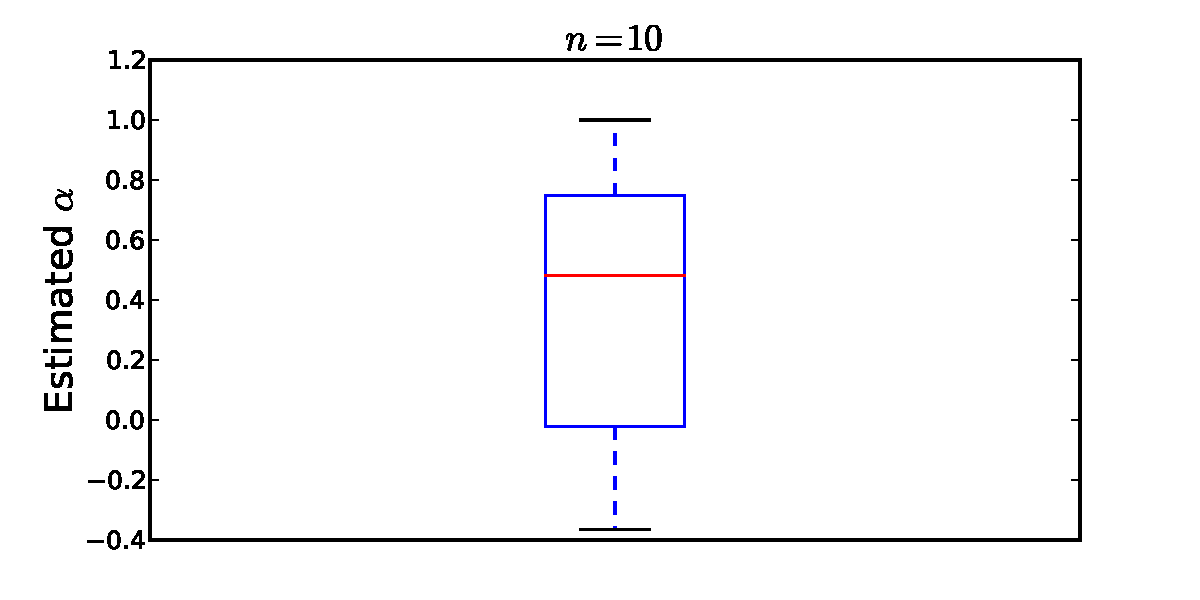
\includegraphics[width=\textwidth]{boxes1}
    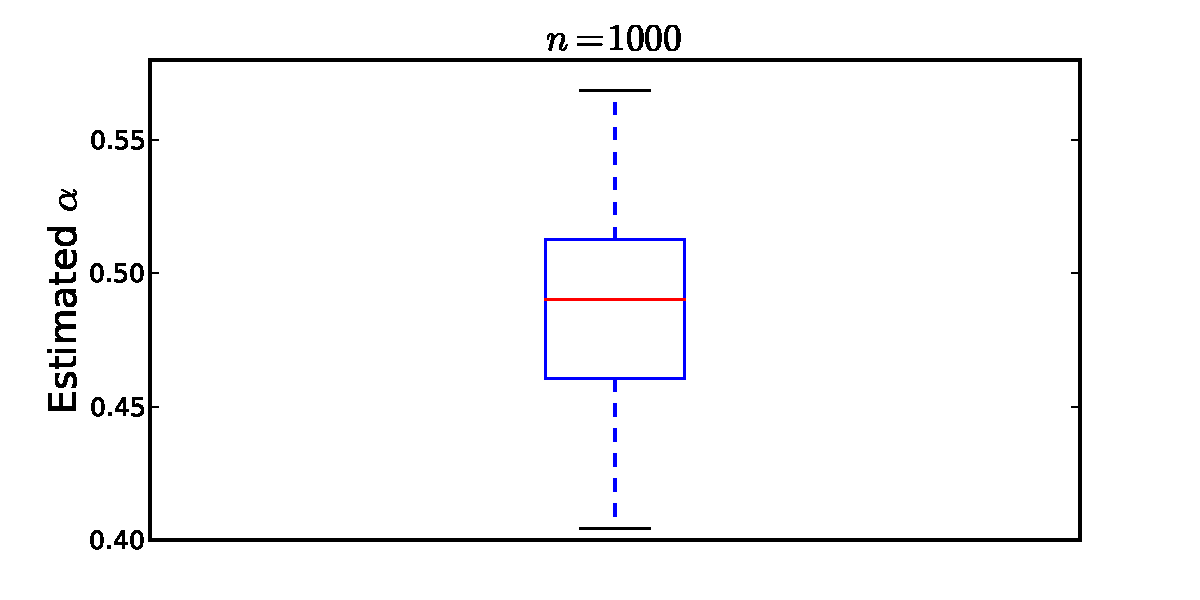
\includegraphics[width=\textwidth]{boxes2}
    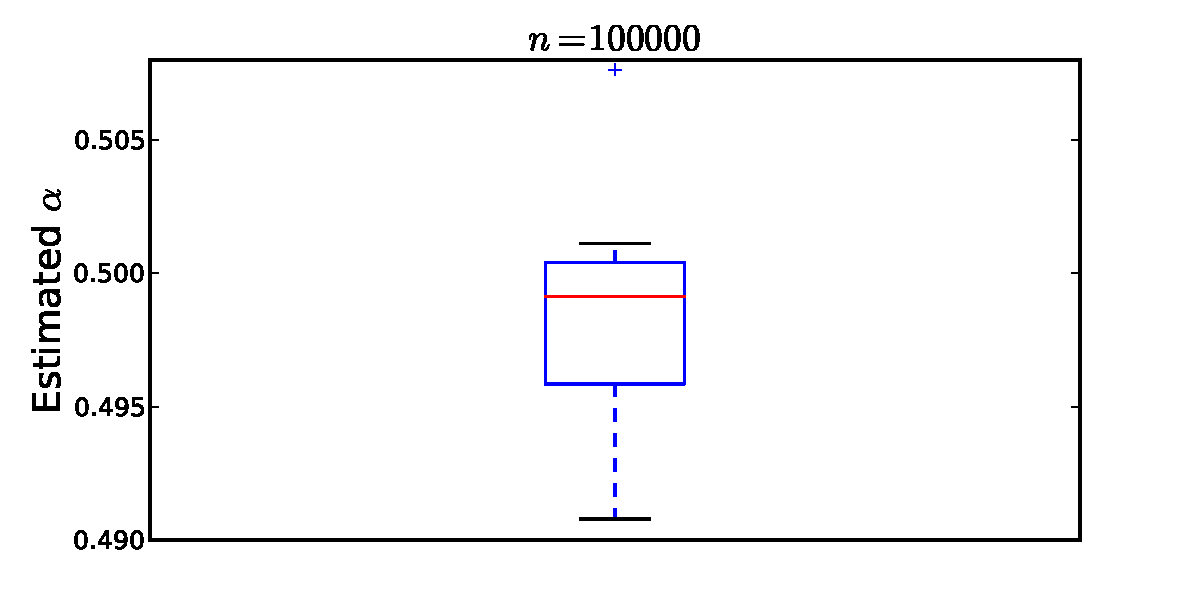
\includegraphics[width=\textwidth]{boxes3}
    \caption{Boxplots for exercise 8.}
\end{figure}


\end{document}

